\begin{figure}[h]\centering
  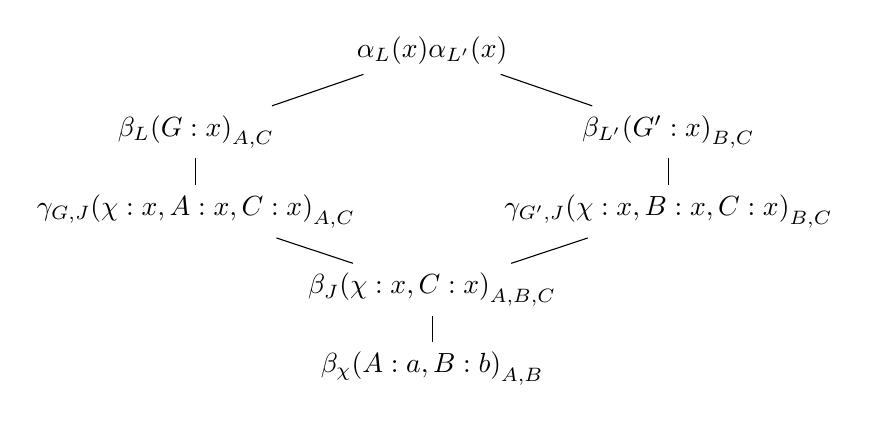
\begin{tikzpicture}[x=3cm,y=1cm]

    % Specification of nodes (position, etc.)
    \node (a0) at (0,0) { $\adj{\alpha_L(x)\alpha_{L'}(x)}$ };
    \node (b0) at (-1,-1) { $\enf{\beta_L(G: x)}_{A, C}$ };
    \node (b1) at (1,-1) { $\enf{\beta_{L'}(G': x)}_{B, C}$ };
    \node (g0) at (-1,-2) { $\enf{\gamma_{G, J}(\chi: x, A: x, C: x)}_{A, C}$ };
    \node (g1) at (1,-2) { $\enf{\gamma_{G', J}(\chi: x, B: x, C: x)}_{B, C}$ };
    \node (j) at (0,-3) { $\enf{\beta_J(\chi: x, C: x)}_{A,B,C}$ };
    \node (c) at (0,-4) { $\enf{\beta_\chi(A: a, B: b)}_{A,B}$ };

    \begin{scope}[-]
      \tikzstyle{every node}=[draw=none,below]
      \draw (a0) to (b0);
      \draw (a0) to (b1);
      \draw (b0) to (g0);
      \draw (b1) to (g1);
      \draw (g0) to (j);
      \draw (g1) to (j);
      \draw (j) to (c);
    \end{scope}

  \end{tikzpicture}
\caption{Ledger channels, $x = a + b$}\label{fig:modes}
\end{figure}
